\section{Method}

\subsection{Compact Student Architecture}

\modelname{} is a pre-activation squeeze-and-excitation residual
network~\cite{he2016identity,hu2018senet} designed for single-channel
$32{\times}32$ images.  Channel widths run $(40, 80, 160)$ across three stages
of depth $(2, 2, 2)$; Stages~2 and~3 downsample by stride~2
(Figure~\ref{fig:arch}).  The total trainable parameter count is
\textbf{1,109,116}.

\begin{figure}[t]
  \centering
  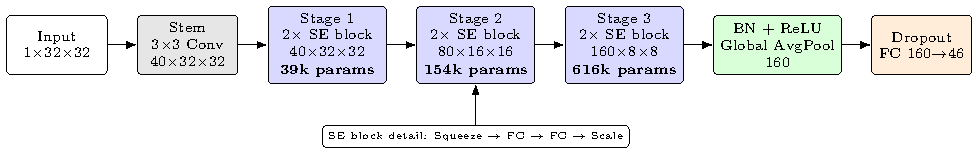
\includegraphics[width=\linewidth]{figures/architecture.pdf}
  \caption{%
    \modelname{} architecture.
    \textbf{(a)}~Full pipeline: a stem convolution feeds three stages of
    PreAct SE-ResBlocks with channel widths $(40, 80, 160)$; a BN--ReLU--GAP
    head produces a 160-dim descriptor before the linear classifier.
    \textbf{(b)}~Unravelled PreAct SE-ResBlock: the main path runs two rounds of
    BN, ReLU, and Conv\,$3{\times}3$.  The SE module then squeezes channel weights
    with a GAP followed by two FCs (ratio $r{=}8$) and a sigmoid; the re-weighted
    features sum with an identity skip (or $1{\times}1$ Conv when downsampling) at~$\oplus$.
  }
  \label{fig:arch}
\end{figure}

\subsection{Teacher Ensemble}

The ensemble comprises 15 teachers drawn from three architecture configurations
crossed with five independent random seeds (seeds 0--4).  Two of those
configurations share widths $(96, 192, 384)$ and depths $(3, 3, 3)$ but differ
in augmentation intensity (medium vs.\ heavy tier; see
Section~\ref{sec:training}); the third uses widths $(64, 128, 256)$ with depths
$(4, 4, 4)$ under medium augmentation.  Parameter counts land at 5.97\,M and
9.89\,M---the spread across configs is intentional, to reduce mode collapse in
the soft targets.  All teachers share the same \modelname{} codebase (the
\texttt{DevNet} class) and are trained without distillation.  Their logits are
dumped once into a single NumPy archive reused across all student runs.

\subsection{Ensemble Knowledge Distillation}
\label{sec:kd}

Following Hinton et al.~\cite{hinton2015distill}, the ensemble target for each
training image is the mean softmax of 9 teacher checkpoints (configs A, B,
C $\times$ seeds 0--2), where each teacher's softmax incorporates
horizontal-flip test-time averaging.  The objective is:
\begin{equation}
  \mathcal{L} = \alpha \cdot T^{2}\,
    \mathrm{KL}\!\left(
      \sigma\!\left(\tfrac{z_{t}}{T}\right) \,\Big\|\,
      \sigma\!\left(\tfrac{z_{s}}{T}\right)
    \right)
    + (1-\alpha)\cdot\mathrm{CE}(z_{s}, y),
  \label{eq:kdloss}
\end{equation}
where $z_{s}$ and $z_{t}$ are student and (mean) teacher logits, $\sigma$
denotes the softmax, $T = 4.0$, and $\alpha = 0.7$.  Label smoothing
($\varepsilon = 0.1$) applies to the hard cross-entropy term.  The KL
is teacher-to-student (teacher as reference distribution).  Target-generation
scheme (clean no-TTA vs.\ flip-averaged) and ensemble size (9 vs.\ 15 teachers)
are ablated in Section~\ref{sec:ablations}.

\subsection{Script-Aware Training}
\label{sec:training}

Devanagari script is not horizontally symmetric: reflecting a glyph produces an
invalid character.  Horizontal flips are excluded entirely.  The training
transform instead applies affine perturbations (rotation, translation, scale,
shear) followed by elastic deformation; an augmentation tier
(\texttt{light}/\texttt{medium}/\texttt{heavy}) selected per configuration
controls the intensity.  Random erasing ($p = 0.25$, area 2--10\%) rounds out
the per-image regularisation.

Mixing augmentations---mixup~\cite{zhang2018mixup} ($\alpha = 0.2$) and
CutMix~\cite{yun2019cutmix} ($\alpha = 1.0$)---are selected with equal
probability, each activated with overall probability 0.5 per batch.  Both are
off during distillation runs: per-image teacher logits cannot be linearly
combined without corrupting the soft-target distribution, so the KD loss
(Equation~\ref{eq:kdloss}) always sees clean, unaugmented teacher predictions.

Optimisation uses AdamW. The learning-rate schedule is cosine with a 5-epoch
linear warm-up.  A weight exponential moving average (EMA, decay 0.999) tracks
a shadow copy; the EMA weights are used for validation and the final checkpoint.

\subsection{Evaluation Protocol}

Reported accuracies come from a single forward pass over the DHCD held-out test
split; no test-time augmentation is applied.  Model selection relies on a 10\%
stratified validation set carved from the training split before any augmentation.

Statistical comparisons between \modelname{} and the baseline~\cite{malla2025}
use the exact two-sided McNemar test~\cite{mcnemar1947} on per-sample binary
correctness indicators.  Confidence intervals for accuracy and error rate are
Wilson score intervals at 95\%~\cite{wilson1927}.  ECE~\cite{guo2017calibration}
is computed with 15 equal-width bins on the held-out test set.
